\documentclass[10pt]{article}
% Эта строка — комментарий, она не будет показана в выходном файле
\usepackage{ucs}
\usepackage[utf8x]{inputenc} % Включаем поддержку UTF8
\usepackage[russian]{babel}  % Включаем пакет для поддержки русского языка
\usepackage{amsmath}
\usepackage{amssymb}
\usepackage{mathtools}

\hoffset=0mm
\voffset=0mm
\textwidth=170mm        % ширина текста
\oddsidemargin=-0mm   % левое поле 25.4 - 5.4 = 20 мм
\textheight=240mm       % высота текста 297 (A4) - 40
\topmargin=-15.4mm      % верхнее поле (10мм)
\headheight=5mm      % место для колонтитула
\headsep=5mm          % отступ после колонтитула
\footskip=8mm         % отступ до нижнего колонтитула



% \textwidth=180mm    
% \oddsidemargin=-10mm 

\title{Лабораторная работа № 3.1.2: {\it Изучение магнитного поля соленоида с помощью датчика Холла.}}
\author{Зотов Алексей, 497}
\date{\today}

\begin{document}

\maketitle
\textbf{Цель работы:} Изучение магнитного поля соленоида, магнитного поля постоянных магнитов, измерение индукции магнитного поля Земли.

\textbf{В работе испольуются:} \small{Соленоид, намотанный на полый цилиндрический каркас, набор из 10 постоянных магнитов в форме дисков ($d = 25$ мм, $h = 5$ мм); 8 небольших одинаковых магнитиков (4х6х8 $\text{мм}^3$), источник постоянного тока с встроенным амперметром, измеритель магнитной индукции Ш1–10 (магнитометр), измеритель магнитной индукции ATE–8702, весы, тонкая нить для изготовления крутильного маятника, секундомер, штангенциркуль, брусок из немагнитного ма- териала 25х30х60 мм3, штатив из немагнитного материала.}

\textbf{Ход работы:}
\paragraph{\large {A. Исследование зависимости индукции магнитного поля на оси соленоида.\\}} 
    \begin{enumerate}
    \item 
        Установим ток в соленоиде $I = 0.5$A, найдем зависисмость $B = B(z)$ индукции магнитного поля от координаты $z$, направленной вдоль оси соленоида.\\
        $B = [1.31, 1.89,2.87,4.34,5.54,6.71,7.42,7.84,8.10,8.20,8.24,8.35,8.34,8.31,8.22,8.05,7.73]$ мТл. \\
        $z = [2, 3, 4, 5, 6, 7, 8, 9, 10, 11, 12, 13, 14, 15, 16, 17, 18]$ см. \\

        \begin{center}
        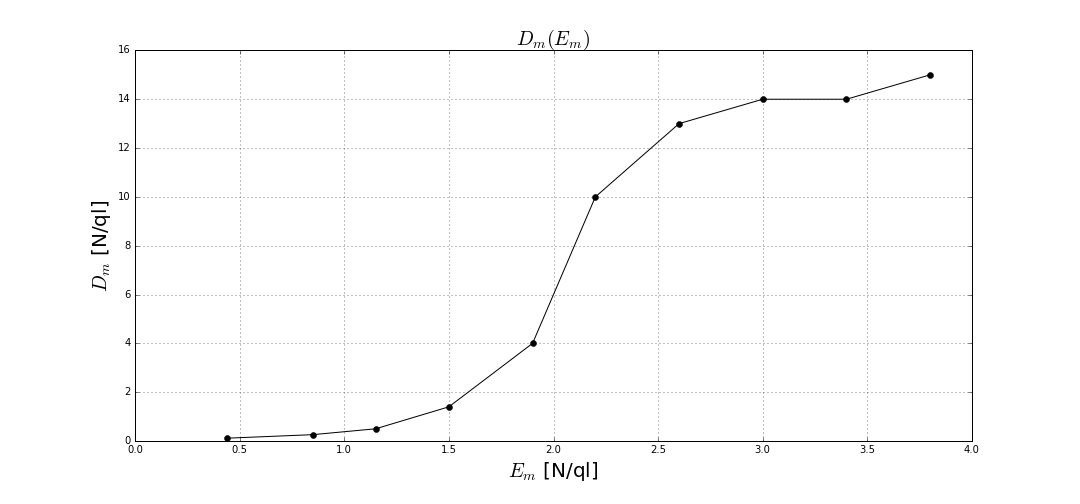
\includegraphics[width=12cm,height=5cm]{plot1.png}
        \end{center}
        Cредняя точка на оси соленоида $z_0 = 13 \pm 0.5$ см.
    \item Установим зонд в среднюю точку $z_0$ и найдем $B = B(I)$ - зависимость индукции от силы тока. \\
            $B = [8.26,11.50,14.72,17.47,20.3,23.4,26.4,29.2,32.1,34.8,38.1]$ мТл. \\
            $I = [0.5, 0.7, 0.9,  1.1,  1.3,  1.5 , 1.7,  1.9 , 2.1 , 2.3 , 2.5]$ А.
            \begin{center}
            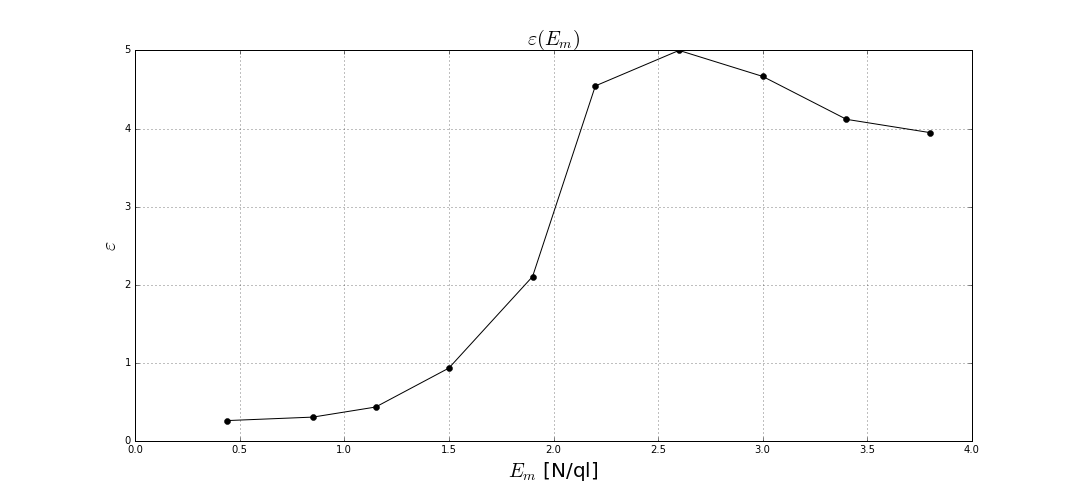
\includegraphics[width=12cm,height=5cm]{plot2.png}
            \end{center}
    \item Сравним полученную зависимость $B(z)$ с теоретической $B = B_{\text{th}}(z)$ \\ 
            Пармаетры соленоида: 
            \begin{enumerate}
                \item число витков $N = 2300$
                \item длина $l = 16.7$
                \item радиус $r = 3.1$
            \end{enumerate}
            Индукция магнитного поля соленоида:
            \begin{equation}
                B = \frac{\mu_0}{4 \pi} 2 \pi In(\cos{\alpha} - \cos{\beta})
            \end{equation} где, $mu_0 = 4 \pi * 10^-7$ Гн / м - магнитная постоянная , $n = N/l$ - плотность намотки, $\alpha$ и $\beta$ углы под которыми видны задний и передний торцы соленоида соответственно. Выражая $\cos{\alpha}$ и $\cos{\beta}$ через $z$, получим :
            \begin{equation}
                cos{\alpha} = \frac{z_2 - z }{ \sqrt{R^2 + (z_2-z)^2}} 
            \end{equation}
            \begin{equation}
                cos{\beta} = \frac{z_1-z}{\sqrt{R^2 + (z_1-z)^2}}  
            \end{equation}
            где $z_1$ и $z_2$ - координаты начала и конца соленоида соответственно. \\
            Определим $z_1$ и $z_2$ экспериментально, по графику $B(z)$ , считая что в точке $z_1$ индукция в 2 раза меньше чем максимальная, а $z_2$ симметрична относительно точки с максимальной индукцией. Возьмем $z_1 = 4.7$см ,
            тогда $z_2 = z_1 + 2(z_0 - z_1) = 21.3$ см. Оценочная длина $l = z_2 - z_1 = 16.6$ , что близко к настоящему значению.\\
            Оценим плотность намотки $n = \frac{B_{\max}}{\mu_0 I}, N = nl$: $n \approx 137.7$ витков/см , $N \approx 2286$.
            \begin{center}
            \includegraphics[width=13cm,height=6cm]{plot12.png}
            \end{center}
            Графики почти совпадают. Теоретическое значение центра соленоида $z_0 = 13.4 \pm 0.3$см , с учетеом погрешности совпадает с экспериментальным результатом.
    \end{enumerate}

\paragraph{\large {Б. Исследование индукции магнитного поля постоянных магнитов.\\}} 
 
Измерим индукцию магнитного поля в центре цилиндра состоящего из постоянных магнитов в форме диска ($h=0.5$см, $r=0.5$см). \\
$B = [387,440,460,466,470,477,482,486]$ мТл. \\
$n = [2, 3, 4, 5, 6, 7, 8, 9]$ 
\begin{center}
        \includegraphics[width=12cm]{plot3.png}
\end{center}
$B_n = \frac{B_r}{2} \frac{nh}{\sqrt{r^2 + (nh)^2}}$ , отсюда найдем $B_r \approx 944.7$мТл - остаточная индукция.


\paragraph{\large {Г. Определение горизонтальной составляющей магнитного поля Земли.\\}}

Измерим период колебаний $n=8$ шариков. Время $k = 20$ колебаний $t = 50.0 \pm 0.5$с, период $t = 2.50 \pm 0.03$с. $m = 0.853$г, $d = 0.6$см. \\
Найдем горизонтальную составляющую магнитного поля земли из формул:
\begin{equation}
T = 2 \pi \sqrt{\frac{J}{P_m B_h}} \implies B_h = \frac{4 \pi^2 J}{T^2 P_m}
\end{equation} 
$J$ найдем, считая соединенные шарики примерно бруском, а $P^1_m$ из:
\begin{equation}
    F = \frac{\mu_0}{4 \pi} 6 P_m^2/l^4 = mg \implies P_m = l^2 \sqrt{\frac{4 \pi mg}{6\mu_0}}
\end{equation}
Для всей стрелки $P_m = 8P^1_m$, отсюда $B_h = 22.2 \pm 1.8$ мкТл. $\varepsilon_T = 0.01$, $\varepsilon_l = 0.04$.\\
$\varepsilon_{B_h} \approx 0.08$.

\end{document}